\documentclass{prova}

\usepackage{amssymb}
\usepackage[inline]{enumitem}

\newcommand{\sen}{\,\mbox{sen}\,}
\newcommand{\tg}{\,\mbox{tg}\,}
\newcommand{\cosec}{\,\mbox{cosec}\,}
\newcommand{\cotg}{\,\mbox{cotg}\,}
\newcommand{\tr}{\,\mbox{tr}\,}
\newcommand{\ds}{\displaystyle}
\newcommand{\ra}{\rightarrow}

\professor{Prof.\@ Adriano Barbosa}
\disciplina{C\'alculo Diferencial e Integral}
\avaliacao{P2}
\curso{Eng.\@ de Alimentos}
\data{19/07/2018}

\begin{document}
	\cabecalho{5}  % o numero 5 indica a qnt de quadros na tabela de nota

	\textbf{Todas as respostas devem ser justificadas.}

	\begin{questionario}
        \q{Calcule o limite: $\ds\lim_{x\ra\infty} x\sen\left(\frac{\pi}{x}\right)$.}
        \q{Cada lado de um quadrado est\'a aumentando a uma taxa de $3$ cm/s. A
            que taxa a \'area do quadrado est\'a aumentando quando sua \'area for $9$ cm$^2$?}
        \q{Se $900$ cm$^2$ de papel\~ao est\'a dispon\'{\i}vel para fabricar uma caixa
            sem tampa e base quadrada, encontre as dimens\~oes da caixa com volume m\'aximo.}
        \q{O gr\'afico de $g$ consiste em duas retas e um semic\'{\i}rculo. Use-o para
            calcular as integrais abaixo.}
            \begin{figure}[h]
                \centering
                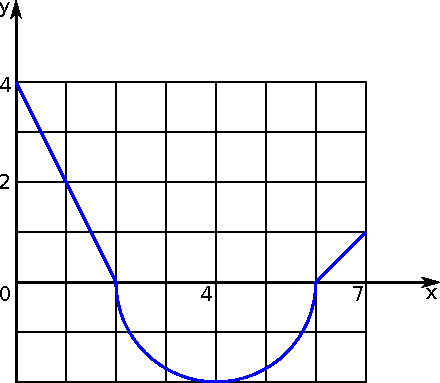
\includegraphics[width=0.4\textwidth]{q4.pdf}
            \end{figure}

            \begin{enumerate*}
                \item $\ds\int_0^2 g(x)\ dx$
                \hspace{0.5cm}
                \hspace{0.5cm}
                \item $\ds\int_2^6 g(x)\ dx$
                \hspace{0.5cm}
                \hspace{0.5cm}
                \item $\ds\int_0^6 g(x)\ dx$
            \end{enumerate*}
        \q{Calcule a integral $\ds\int_0^1(x+1)(x-2)\ dx$.}
	\end{questionario}
\end{document}
